% --------------------------------------
% Document Class
% --------------------------------------
\documentclass[a4paper,11pt]{article}
% --------------------------------------



% --------------------------------------
% Use Package
% --------------------------------------


\usepackage[francais]{babel}
%\usepackage{ucs}
\usepackage[utf8]{inputenc}
\usepackage[T1]{fontenc}

\usepackage{makeidx}
\usepackage{color}
\usepackage{graphicx}
\usepackage{float}
\usepackage[hidelinks]{hyperref} 
\usepackage{geometry}
%\usepackage{lastpage}
%\usepackage{marginnote}
\usepackage{fancyhdr}
%\usepackage{titlesec}
%\usepackage{framed}
\usepackage{amsmath}
\usepackage{empheq}
\usepackage{array}
\usepackage{multicol}
%\usepackage{adjustbox}

% insert code
\usepackage{listings}

% define our color
\usepackage{xcolor}

% code color
\definecolor{ligthyellow}{RGB}{250,247,220}
\definecolor{darkblue}{RGB}{5,10,85}
\definecolor{ligthblue}{RGB}{1,147,128}
\definecolor{darkgreen}{RGB}{8,120,51}
\definecolor{darkred}{RGB}{160,0,0}

% other color
\definecolor{ivi}{RGB}{141,107,185}


\lstset{
    language=Scilab,
    captionpos=b,
    extendedchars=true,
    frame=lines,
    numbers=left,
    numberstyle=\tiny,
    numbersep=5pt,
    keepspaces=true,
    breaklines=true,
    showspaces=false,
    showstringspaces=false,
    breakatwhitespace=false,
    stepnumber=1,
    showtabs=false,
    tabsize=3,
    basicstyle=\small\ttfamily,
    backgroundcolor=\color{ligthyellow},
    keywordstyle=\color{ligthblue},
    morekeywords={include, printf, uchar},
    identifierstyle=\color{darkblue},
    commentstyle=\color{darkgreen},
    stringstyle=\color{darkred},
}


% --------------------------------------



% --------------------------------------
% Page setting
% --------------------------------------
%\pagestyle{empty}
\setlength{\headheight}{15pt}

\setcounter{secnumdepth}{3}
\setcounter{tocdepth}{2}

\makeatletter
\@addtoreset{chapter}{part}
\makeatother 

\hypersetup{         % parametrage des hyperliens
  colorlinks=true,      % colorise les liens
  breaklinks=true,      % permet les retours à la ligne pour les liens trop longs
  urlcolor= blue,       % couleur des hyperliens
  linkcolor= black,     % couleur des liens internes aux documents (index, figures, tableaux, equations,...)
  citecolor= green      % couleur des liens vers les references bibliographiques
}

% --------------------------------------

% --------------------------------------
% Information
% --------------------------------------
\title{Compte-rendu TP7 Rdf : Réduction de la dimension par analyse en composantes principales et analyse factorielle discriminante}
\author{Elliot VANEGUE et Gaëtan DEFLANDRE}
% --------------------------------------

\definecolor{myColor}{rgb}{0.5, 0.1, 0.75}

% --------------------------------------
% Begin content
% --------------------------------------
\begin{document}

% Set language to english
  \selectlanguage{francais}

  % Start the page counting
  \pagenumbering{arabic}

  \maketitle
  
  \mbox{}
  \newpage
  \clearpage
  
  \section*{Introduction}
  Lors de ce TP, nous cherchons à passer d'une représentation de la classification de données
  bi-dimensionnelle à une représentation mono-dimensionnelle. Pour cela, nous nous servons de
  deux méthode : l'analyse en composantes principales et l'analyse factorielle discriminante.
  Afin de déterminer la méthode la plus performante pour notre cas d'étude, nous avons classifié
  les données projeté avec une analyse linéaire discriminante.
 
  \section{Données d'apprentissage}
  Dans un premier temps, nous avons affiché les données d'apprentissage et les données de test.
  
  \begin{figure}[H]
    \center
   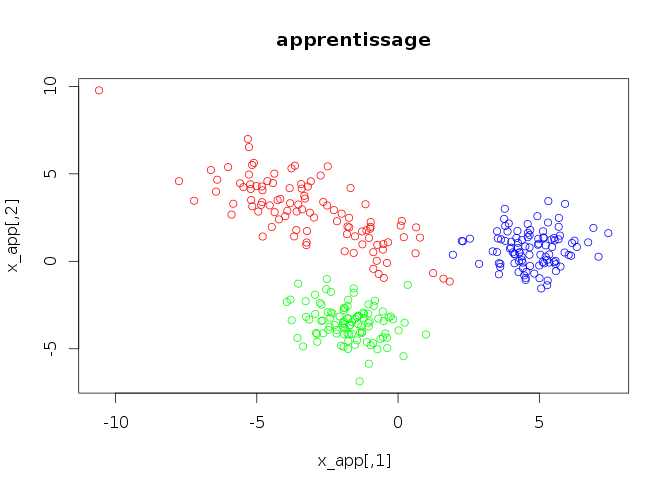
\includegraphics[width=8cm]{donnees_apprentissage.png}
   \caption{Graphique des données d'apprentissage}
  \end{figure}
  
  Nous pouvons voir que les données sont regroupé par classe pour les données d'apprentissage.
  
  \begin{figure}[H]
  \center
   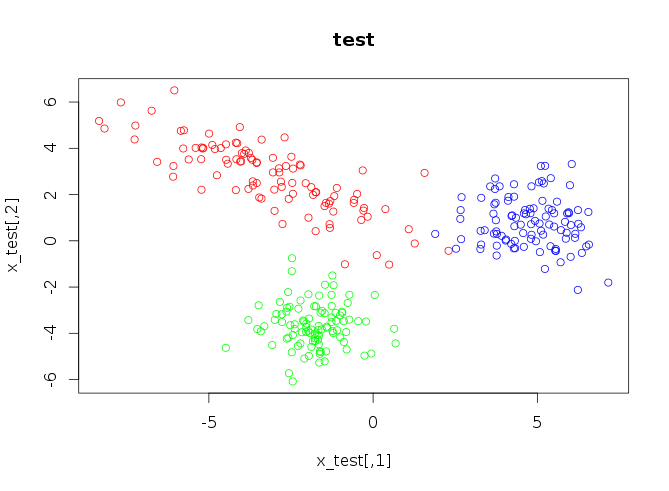
\includegraphics[width=8cm]{donnees_test.png}
   \caption{Graphique des données de test}
  \end{figure}
  
  Les données de test adopte le même comportement que les données d'apprentissage.
  
  \section{Analyse en composantes principale}
  
  Tout d'abord, nous calculons la co-variance des données d'apprentissage dans le but de déterminer
  l'axe le plus adapté à l'analyse des données. Nous déterminons cette axe en prenant comme vecteur
  le vecteur propre de la valeur propre la plus élevé.\\
  
  \begin{lstlisting}[caption=Calcule de l'axe discriminant]
  Vp <- eigen(covariance)

  #affichage de la pente
  pente <- Vp$vectors[2,1]/Vp$vectors[1,1]
  abline(a = 0, b = pente, col = "blue")
  \end{lstlisting}

  Le but de cette démarche est de projeter les données étudiées sur cette droite. Pour cela, il
  faut calculer le vecteur de chaque donnée qui va permettre de positionner celle-ci sur l'axe 
  discriminant.\\
  
  \begin{lstlisting}[caption=Projection des données d'apprentissage sur l'axe discriminant]
  #produit scalaire
  ScalarProduct_app <- x_app
  ScalarProduct_app <- x_app %*% (Vp$vectors[,1] / sqrt(sum(Vp$vectors[,1]*Vp$vectors[,1])))

  #projection des points
  x_app_ACP <- x_app
  x_app_ACP[,1] = ScalarProduct_app * Vp$vectors[1,1]
  x_app_ACP[,2] = ScalarProduct_app * Vp$vectors[2,1]
  \end{lstlisting}
  
  \begin{figure}[H]
  \center
   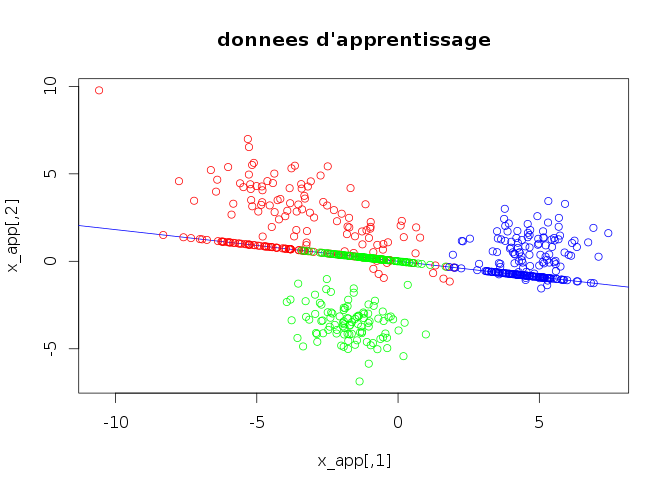
\includegraphics[width=9cm]{apprentissage_acp.png}
   \caption{Graphique des données d'apprentissage projeté sur la droite}
  \end{figure}
  
  Nous pouvons voir sur ce graphique qu'il y a une zone sur l'axe discriminant où il y de nombreuses
  données de la classe rouge qui sont projetées au même endroit que des données de la classe verte.
  Cela risque de provoquer quelques erreurs lors de la classification des données.
  
  \subsection{Classification par analyse linéaire discriminante}
  
  Nous pouvons maintenant classer les données projetées grâce à une analyse linéaire discriminante. Nous 
  déterminons grâce à cette analyse que le taux d'erreur de la classification des données est de 84\%.
  
  \begin{figure}[H]
  \center
   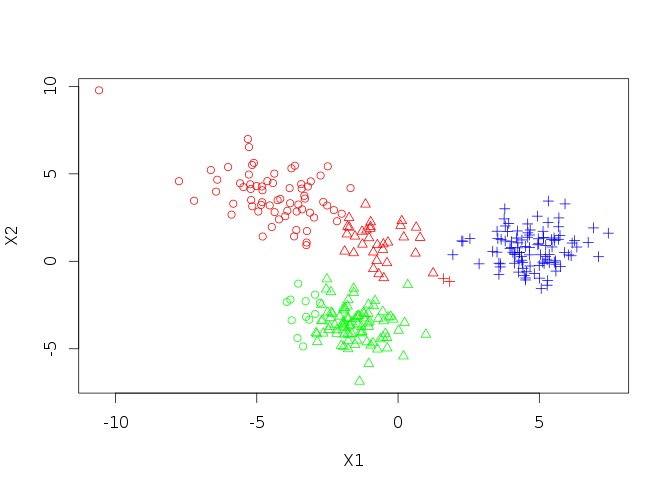
\includegraphics[width=9cm]{apprentissage_classifie.png}
   \caption{Graphique des données d'apprentissage classifié par analyse linéaire discriminante}
  \end{figure}

  Nous avons créé un tableau contenant la position des données afin de connaître quels classes
  comportent le plus d'erreur de classification. Les données sont alors classifié de la manière suivante :
  \begin{center}
  \begin{tabular}{|c|c|c|c|}
   \hline
   classe & R & V & B\\
   \hline
   R & 66 & 32 & 2 \\
   \hline
   V & 12 & 88 & 0 \\
   \hline
   B & 0 & 0 & 100 \\
   \hline
  \end{tabular}
  \end{center}

  On peut voir dans ce tableau qu'il n'y a aucune erreur sur la classe bleu. En revanche, il n'y a que 66\%
  de données de la classe rouge qui sont correcte.\\
  
  Nous avons effectué la même classification avec les données tests. Nous obtenons un taux de bonne classification
  de 87\%.
  
  \begin{figure}[H]
  \center
  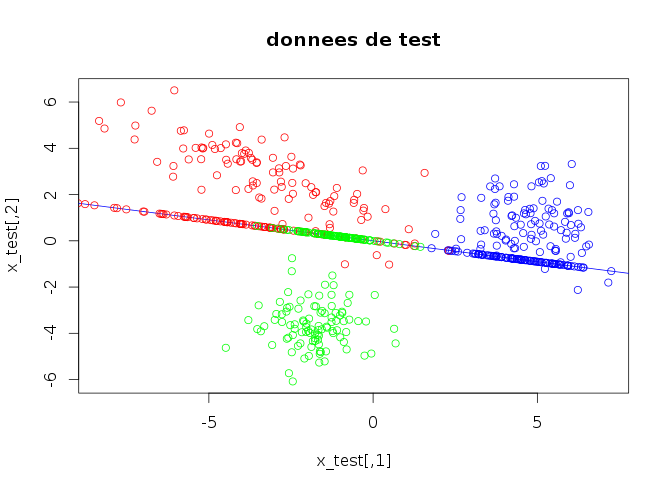
\includegraphics[width=9cm]{test_acp.png}
   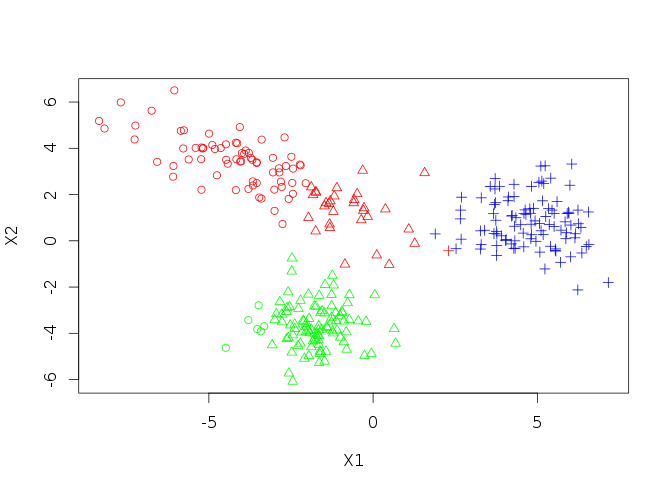
\includegraphics[width=9cm]{test_classifie.png}
   \caption{Graphique des données de test classifié par analyse linéaire discriminante}
  \end{figure}
  
  Les données sont alors classifié de la manière suivante :
  \begin{center}
  \begin{tabular}{|c|c|c|c|}
   \hline
   classe & R & V & B\\
   \hline
   R & 69 & 30 & 1 \\
   \hline
   V & 6 & 94 & 0 \\
   \hline
   B & 0 & 0 & 100 \\
   \hline
  \end{tabular}
  \end{center}
  
  Les résultats sont à peu prêt équivalant aux données d'apprentissage, c'est à nouveau la classe rouge
  qui à le plus grand taux d'erreur. Les résultats de cette classification sont trop juste car les erreurs
  de classification se concentre sur une classe plus que sur les deux autres dans notre exemple.
  
  \section{Analyse factorielle discriminante}
  
  Le but de cette méthode est de rechercher l'attribut qui maximise la distance entre
  les moyennes de chaque classe et minimise la dispersion intra-classe. Pour cela nous
  devons d'abord calculer les matrices dispersion intra et inter-classe.
  
  \subsection{Estimation des moyennes et co-variances des classes}
  Nous allons dans un premier temps estimer la moyenne de chaque classe dans le but
  de calculer la matrice dispersion inter-classe. Nous obtenons la moyenne de chaque 
  classe avec la macro suivante : 
  
  \begin{lstlisting}
    mean1 <- colMeans(x_app[classe_app==1,])
    mean2 <- colMeans(x_app[classe_app==2,])
    mean3 <- colMeans(x_app[classe_app==3,])
  \end{lstlisting}

  Nous pouvons alors calculer la matrice dispersion inter-classe de la manière suivante :
  
  \begin{lstlisting}
    Sb=(mean1-mean)%*%t(mean1-mean)+
      (mean2-mean)%*%t(mean2-mean)+
      (mean3-mean)%*%t(mean3-mean)
  \end{lstlisting}
  
  Pour la matrice dispersion intra-classe, nous calculons la matrice de co-variance de chaque
  classe, puis nous calculons la matrice dispersion comme ce-ci : 
  
  \begin{lstlisting}
    Sw=S1+S2+S3
  \end{lstlisting}
  
  Il reste à calculer l'équation de la droite avec la macro suivante : 
  
  \begin{lstlisting}
    invSw= solve(Sw)
    invSw_by_Sb= invSw %*% Sb
    Vp<- eigen(invSw_by_Sb)
  \end{lstlisting}
  
  Nous obtenons le résultat suivant : 
  
  \begin{figure}[H]
  \center
   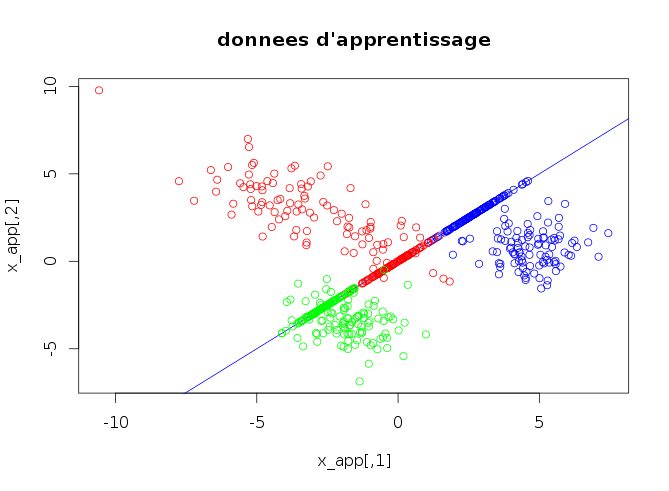
\includegraphics[width=9cm]{app_fact.png}
   \caption{Graphique des données d'apprentissage après analyse factorielle discriminante}
  \end{figure}
  
  On voit que l'axe disciminant possède une pent plus importante que dans une analyse en 
  composantes principales. Cela permet une meilleur séparation des classes rouge et verte, car
  on peu voir que les projetés des données de la classe verte sont beaucoup moins mélangé 
  que dans l'analyse précédente. Pour vérifier cela, nous avons effectué une analyse linéaire
  discriminante, ce qui nous donne un taux de bonne classification de 97\%, ce qui est bien
  meilleur qu'une analyse en composantes principales. 
  
  \begin{figure}[H]
    \center
   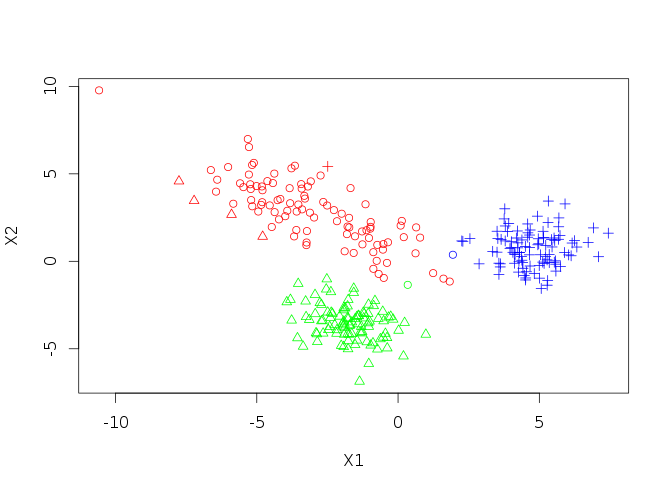
\includegraphics[width=9cm]{app_fact_class.png}
    \caption{Classification des données d'apprentissage après analyse factorielle discriminante}
  \end{figure}

  Voici la table de classification de ces 
  données : \\
  
  \begin{center}
  \begin{tabular}{|c|c|c|c|}
   \hline
   classe & R & V & B\\
   \hline
   R & 95 & 4 & 1 \\
   \hline
   V & 1 & 99 & 0 \\
   \hline
   B & 2 & 0 & 98 \\
   \hline
  \end{tabular}
  \end{center}
  
  On voit que les erreurs que nous avions précédemment avec la classe rouge on était grandement
  diminué.\\
  
  Nous avons effectué les mêmes analyses sur les données de test. Le taux de bonne classification de ces 
  données est de 96\%. La encore l'analyse factorielle fournit de meilleur résultat que l'analyse en composante
  principale.\\
  
  \begin{figure}[H]
    \center
   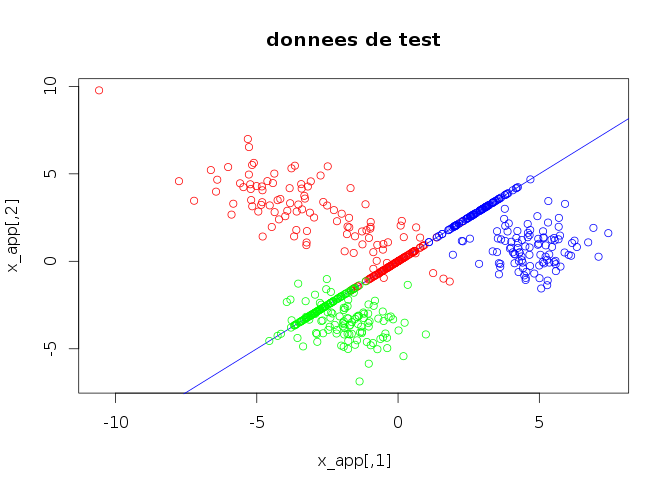
\includegraphics[width=9cm]{test_fact.png}
    \caption{Graphique des données de test après analyse factorielle discriminante}
  \end{figure}
  
   \begin{figure}[H]
    \center
   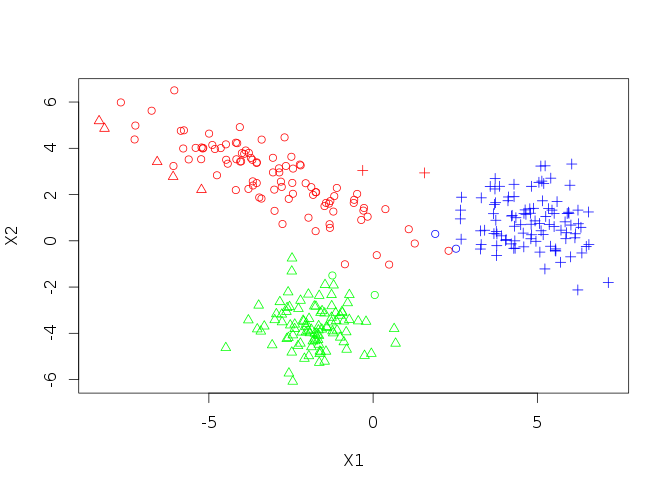
\includegraphics[width=9cm]{test_fact_class.png}
    \caption{Classification des données de test après analyse factorielle discriminante}
  \end{figure}
  
  \begin{center}
  \begin{tabular}{|c|c|c|c|}
   \hline
   classe & R & V & B\\
   \hline
   R & 93 & 5 & 2 \\
   \hline
   V & 2 & 98 & 0 \\
   \hline
   B & 2 & 0 & 98 \\
   \hline
  \end{tabular}
  \end{center}
  
  %Q9 plus ou moin fait lorsqu'on parle de la pente de la courbe
  \section{Comparaison classification dans l'espace d'origine bi-dimensionnel vs sur le premier axe}
  Maintenant que nous connaissons les taux de bonne classification sur le premier axe, nous allons
  les comparer à ceux de l'espace d'origine. Nous obtenons un taux de bonne classification dans l'espace
  d'origine de 99\%.
  
   \begin{figure}[H]
    \center
   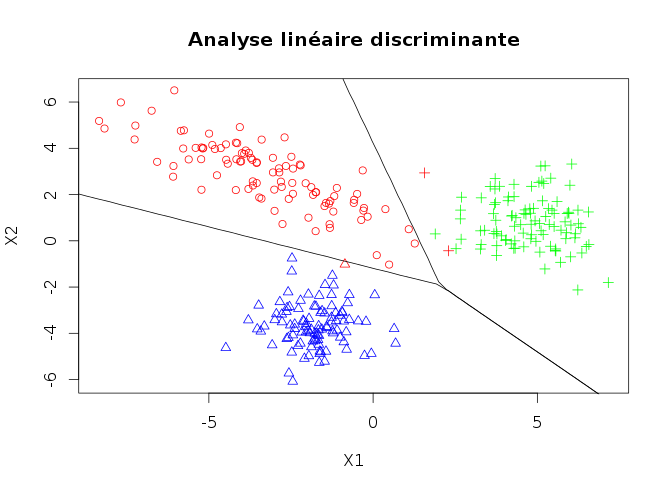
\includegraphics[width=9cm]{analyse_lin_test.png}
    \caption{Analyse linéaire discriminante sur l'espace d'origine}
  \end{figure}
  
  %TODO question 10 a voir
  
  \section{Conclusion}
  %TODO
  
  \newpage
  \section{Annexe}
  \begin{lstlisting}[caption=Macro de l'analyse en composante principale]
  (load(file='x_app.data'))
  (load(file='classe_app.data'))
  (load(file='x_test.data'))
  (load(file='classe_test.data'))

  n_test <- 300

  couleur<-rep('red',n_test)
  couleur[classe_test==2]='green'
  couleur[classe_test==3]='blue'

  plot(x_test, col = couleur, main="donnees d'apprentissage")

  #calcul de la covariance
  covariance <- cov(x_test)
  print("matrice de la covariance")
  print(covariance)

  Vp <- eigen(covariance)

  #affichage de la pente
  pente <- Vp$vectors[2,1]/Vp$vectors[1,1]
  abline(a = 0, b = pente, col = "blue")

  #produit scalaire
  ScalarProduct_test <- x_test
  ScalarProduct_test <- x_test %*% (Vp$vectors[,1] / sqrt(sum(Vp$vectors[,1]*Vp$vectors[,1])))

  #projection des points
  x_test_ACP <- x_test
  x_test_ACP[,1] = ScalarProduct_test * Vp$vectors[1,1]
  x_test_ACP[,2] = ScalarProduct_test * Vp$vectors[2,1]

  #affichage des points projetes
  points(x_test_ACP[classe_test==1,], col="red")
  points(x_test_ACP[classe_test==2,], col="green")
  points(x_test_ACP[classe_test==3,], col="blue")

  #////////////////// ALD ///////////////////////
  x_app_ACP.lda<-lda(ScalarProduct_test, classe_app)
  assigne_app<-predict(x_app_ACP.lda, newdata = ScalarProduct_test)
  # Estimation des taux de bonnes classifications
  table_classification_app <-table(classe_app, assigne_app$class)
  print("matrice de confusion :")
  print(table_classification_app)

  # table of correct class vs. classification
  diag(prop.table(table_classification_app, 1))
  # total percent correct
  taux_bonne_classif_app <-sum(diag(prop.table(table_classification_app)))
  print(paste("taux de bonne classification", taux_bonne_classif_app))

  # forme : les classe d'assignation fournie par l'ALD
  shape<-rep(1,n_app)
  shape[assigne_app$class==2]=2
  shape[assigne_app$class==3]=3
  # Affichage des projections apprentissage classees
  plot(x_test,col=couleur2,pch=shape,xlab = "X1", ylab = "X2")

  \end{lstlisting}
  
  \begin{lstlisting}[caption=Macro de l'analyse en composante principale]
  (load(file='x_app.data'))
  (load(file='classe_app.data'))
  (load(file='x_test.data'))
  (load(file='classe_test.data'))

  n_app <- 300

  couleur<-rep('red',n_app)
  couleur[classe_app==2]='green'
  couleur[classe_app==3]='blue'

  plot(x_test, col = couleur, main="donnees de test")

  # moyenne classe1
  mean <- colMeans(x_app)
  mean1 <- colMeans(x_app[classe_app==1,])
  mean2 <- colMeans(x_app[classe_app==2,])
  mean3 <- colMeans(x_app[classe_app==3,])

  print(paste("mean : ", mean))
  print(paste("mean 1 : ", mean1))
  print(paste("mean 2 : ", mean2))
  print(paste("mean 3 : ", mean3))
  # covariance intra-classe classe 1
  S1 <- cov(x_app[classe_app==1,])
  S2 <- cov(x_app[classe_app==2,])
  S3 <- cov(x_app[classe_app==3,])

  Sw=S1+S2+S3
  # covariance inter-classe
  Sb=(mean1-mean)%*%t(mean1-mean)+
    (mean2-mean)%*%t(mean2-mean)+
    (mean3-mean)%*%t(mean3-mean)

  # Resolution equation
  invSw= solve(Sw)
  invSw_by_Sb= invSw %*% Sb
  Vp<- eigen(invSw_by_Sb)

  # Affichage de la droite correspondant au vecteur propre
  # dont la valeur propre la plus elevee
  pente <- Vp$vectors[2,1]/Vp$vectors[1,1]
  abline(a = 0, b = pente, col = "blue")

  #produit scalaire
  ScalarProduct_test <- x_test
  ScalarProduct_test <- x_test %*% (Vp$vectors[,1] / sqrt(sum(Vp$vectors[,1]*Vp$vectors[,1])))

  #projection des points
  x_test_ACP <- x_test
  x_test_ACP[,1] = ScalarProduct_test * Vp$vectors[1,1]
  x_test_ACP[,2] = ScalarProduct_test * Vp$vectors[2,1]

  #affichage des points projetes
  points(x_test_ACP[classe_test==1,], col="red")
  points(x_test_ACP[classe_test==2,], col="green")
  points(x_test_ACP[classe_test==3,], col="blue")

  #////////////////// ALD ///////////////////////
  x_app_ACP.lda<-lda(ScalarProduct_test, classe_app)
  assigne_app<-predict(x_app_ACP.lda, newdata = ScalarProduct_test)
  # Estimation des taux de bonnes classifications
  table_classification_app <-table(classe_app, assigne_app$class)
  print("matrice de confusion :")
  print(table_classification_app)

  # table of correct class vs. classification
  diag(prop.table(table_classification_app, 1))
  # total percent correct
  taux_bonne_classif_app <-sum(diag(prop.table(table_classification_app)))
  print(paste("taux de bonne classification", taux_bonne_classif_app))

  # forme : les classe d'assignation fournie par l'ALD
  shape<-rep(1,n_app)
  shape[assigne_app$class==2]=2
  shape[assigne_app$class==3]=3
  # Affichage des projections apprentissage classees
  plot(x_test,col=couleur,pch=shape,xlab = "X1", ylab = "X2")

  \end{lstlisting}

\end{document}  